\documentclass[xcolor=dvipsnames]{beamer}

% ==== 主題 ====
\usetheme{metropolis}
\usefonttheme{professionalfonts}          % 不覆蓋你自訂的字型

% ==== 字型 ====
\usepackage{fontspec}
\usepackage{xeCJK}
\renewcommand{\familydefault}{\rmdefault} % 使用 serif 字體（重點）
\usefonttheme{professionalfonts}

% 西文字型：Times New Roman 的開源替代品
\setmainfont{TeX Gyre Termes}[
  Ligatures=TeX,
  BoldFont={* Bold},
  ItalicFont={* Italic}
]

% 中文字型（可改為思源宋體、標楷體等）
\setCJKmainfont{Noto Serif CJK TC}
\setCJKsansfont{Noto Sans CJK TC} % 有需要再用
\setCJKmonofont{Noto Sans Mono CJK TC}

% ==== 數學字型（與正文字體一致）====
\usepackage{unicode-math}
\setmathfont{TeX Gyre Termes Math}

% ==== 套件 ====
\usepackage{amsmath, amssymb}
\usepackage{graphicx}
\usepackage{hyperref}
\usepackage{minted}
\usepackage{fvextra}
\usepackage{xcolor}
\usepackage{booktabs}

% ==== 顏色設定（可選）====
\definecolor{MyBlue}{RGB}{3, 55, 105}
\setbeamercolor{structure}{fg=MyBlue}
\setbeamercolor{block title}{bg=MyBlue,fg=white}
\setbeamercolor{block body}{bg=blue!5}
\setbeamertemplate{section in toc}{%
  \inserttocsectionnumber.~\inserttocsection\par
}

\setminted{
    linenos,                % 行號
    frame=lines,            % 上下框線
    framesep=5pt,           % 程式碼與邊框距離
    numbersep=8pt,          % 行號與程式碼距離
    fontsize=\scriptsize,   % 字體大小
    breaklines,             % 自動換行
    tabsize=4,              % tab 寬度
    rulecolor=\color{black},% 框線顏色
    xleftmargin=1.5em       % 左側縮排
}

\title{Stack and Queue}
\author{Tai, Wei Hsuan}
\date{week 6}

\begin{document}
	\begin{frame}
		\titlepage
	\end{frame}

    \begin{frame}
        \frametitle{\href{https://drive.google.com/drive/folders/1IN7Dv6ozKHldRXJG6mI0DmjhBlwO6KWK?usp=sharing}{課程簡報}}
        \begin{figure}
            \centering
            
\includegraphics[width=0.7\textwidth]{src/qrcode.png}
        \end{figure}
    \end{frame}

    \begin{frame}
        \frametitle{Outline}
        \tableofcontents
    \end{frame}
    \section{Recap Problems}
    \section{Stack}
    \begin{frame}{What is stack?}
        In English, stack means "a pile of things arranged one on top of another(Cambridge Dictionary)". In C++, stack is a container adapter that gives the programmer the functionality of a stack data structure. 
    \end{frame}

    \begin{frame}{How a stack works?}
        Stack is a Last In First Out (LIFO) data structure. The last element added to the stack will be the first one to be removed.
        
        In other words, you can only access the top element of the stack(i.e., the most recently added element). You can push elements onto the stack, remove elements from the stack, and check the top element of the stack.
        \begin{figure}
            \centering
            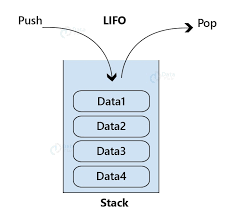
\includegraphics[width=0.5\textwidth]{src/stack.png}
        \end{figure}
    \end{frame}
    \begin{frame}[fragile]
        \frametitle{Basic usage of stack}
        \begin{minted}{c++}
            //create a stack of TYPE named s:
            stack<TYPE> s;
            //add an element to the top of the stack:
            s.push(ELEMENT);
            //remove the top element of the stack:
            s.pop();
            //access the top element of the stack:
            s.top();
            //access the number of elements in the stack:
            s.size();
            //check if the stack is empty:
            s.empty();
        \end{minted}
        If you want to access the top element of the stack or remove the top element of the stack, you should first check if the stack is empty to avoid runtime errors.
    \end{frame}
    \begin{frame}[fragile]
        \frametitle{Here are some common operations of stack}
        \begin{minted}{c++}
            stack<int> s; //create a stack of integers
            s.push(1); //push 1 onto the stack
            s.push(2); //push 2 onto the stack
            cout<<s.top(); //print the top element of the stack
            s.pop(); //remove the top element of the stack
        \end{minted}
    \end{frame}


    \section{Queue}
    \begin{frame}
        \frametitle{What is queue?}
        In English, queue means "a line of people, usually standing or in cars, waiting for something, or a lot of people who want something(Cambridge Dictionary)". In C++, queue is a container that gives the programmer the functionality of a queue data structure.
    \end{frame}
    \begin{frame}
        \frametitle{How a queue works?}
        Queue is a First In First Out (FIFO) data structure. The first element added to the queue will be the first one to be removed.
        
        In other words, you can only access the front and rear elements of the queue. You can push elements to the rear of the queue, remove elements from the front of the queue, and check the front and rear elements of the queue.
        \begin{figure}
            \centering
            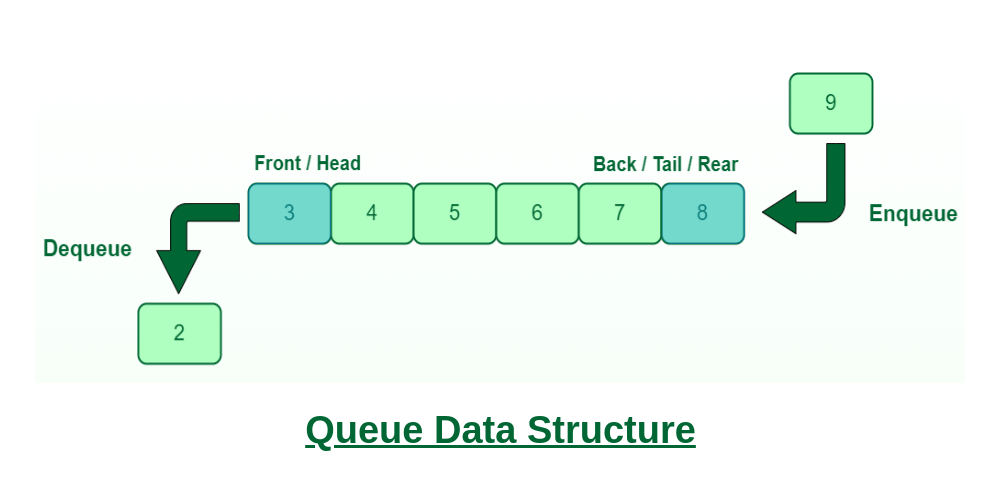
\includegraphics[width=0.7\textwidth]{src/queue.png}
        \end{figure}
    \end{frame}
    \begin{frame}[fragile]
        \frametitle{Basic usage of queue}
        \begin{minted}{c++}
            //create a queue of TYPE named q:
            queue<TYPE> q;
            //add an element to the rear of the queue:
            q.push(ELEMENT);
            //remove the front element of the queue:
            q.pop();
            //access the front element of the queue:
            q.front();
            //access the rear element of the queue:
            q.back();
            //access the number of elements in the queue:
            q.size();
            //check if the queue is empty:
            q.empty();
        \end{minted}
        If you want to access or remove any elements in the queue, you should first check if the queue is empty to avoid runtime errors.
    \end{frame}
    \begin{frame}
        \frametitle{Stack vs Queue}
        \begin{figure}
            \centering
            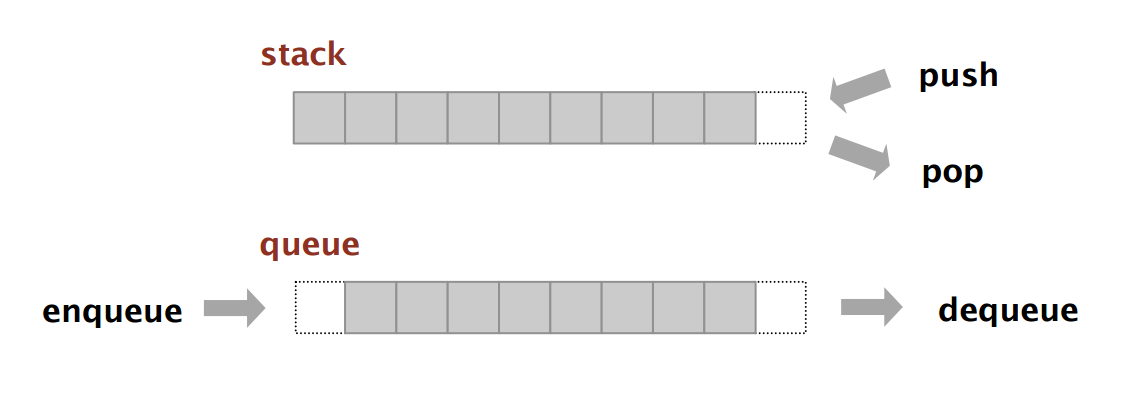
\includegraphics[width=\textwidth]{src/queue_vs_stack.png}
        \end{figure}
    \end{frame}
    \section{Practice Problems}
    \begin{frame}
        \frametitle{Problems}
        Please refer to \textbf{week 6 Stack \& Queue} on zerojudge.
        \begin{itemize}
            \item Basic Stack Problems: i213, a565
            \item Basic Queue Problems: e447
            \item Advanced Stack Problems: c700, j607, r395
            \item Advanced Queue Problems: d718
        \end{itemize}
        I'll mainly focus on the basic problems, the advanced problems are optional.
    \end{frame}

\end{document}